\chapter{Introdução}
A primeira fechadura de que se tem notícia (Figura ~\ref{fig:egipcia})
data de 4000 A.C e foi criada no Egito. Se tratavam de dispositivos de
madeira (seu maior defeito) que podiam ser abertos por grandes chaves
também feitas de madeira. O funcionamento também era parecido com o de
hoje em dia, a chave movia pequenos pistões que ficavam dentro da fechadura.
O grande problema era que o material era muito fácil de ser rompido,
diminuindo assim a segurança \cite{cordeiro2018}

\FloatBarrier
\begin{figure}[!htbp]
	\centering
	\caption{Fechadura egípcia}
	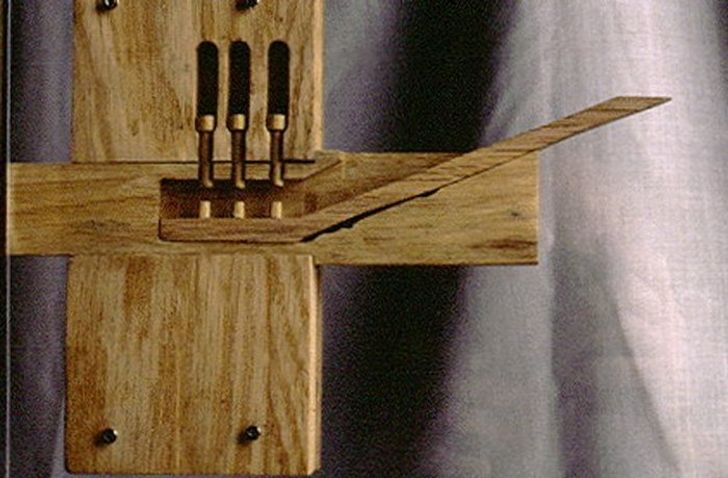
\includegraphics[scale=.2]{imagens/egipcia}
	\\\textbf{Fonte:} \href{https://incrivel.club/admiracao-curiosidades/8-coisas-que-os-antigos-egipcios--faziam-muitos-antes--do-resto-do-mund-327860/}{Incrível}
	\label{fig:egipcia}
\end{figure}
\FloatBarrier

Por isso, com a habilidade no manuseio de metais, como ferro
e bronze, os romanos utilizaram a mesma ideia e a adaptaram para
serem feitas tanto as chaves quanto as fechaduras de metais  isso
aumentou ainda mais a segurança e permitiu uma diminuição no
tamanho de ambos \cite{reprizzo2018}.

Ainda assim, a primeira patente de uma fechadura foi realizada no século XIX
pelo médico Abraham Stransbury. E modelo de fechaduras utilizado hoje (Figura ~\ref{fig:yale})
em dia, com a chave plana e dentada, foi criado por Linus Yale Jr. em 1861 \cite{canabarro2019}.

\FloatBarrier
\begin{figure}[!htbp]
	\centering
	\caption{Fechadura de Yale}
	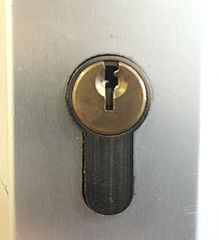
\includegraphics[scale=.4]{imagens/yale}
	\\\textbf{Fonte:} \href{https://pt.wikipedia.org/wiki/Fechadura_de_tambor_de_pinos}{Wikipédia}
	\label{fig:yale}
\end{figure}
\FloatBarrier

Hoje em dia, por mais que o modelo de Yale ainda seja utilizado, devido ao avanço
da tecnologia, principalmente da eletrônica, o uso de fechaduras mais modernas se torna
comum. Assim surgem os modelos elétricos e eletrônicos.


A fechadura elétrica (Figura ~\ref{fig:eletrica}) é mais simples, controlada por
um botão que a abre devido a passagem de corrente elétrica por um solenoide.
Por outro lado, a eletrônica é mais complexa e pode ser feita de vários jeitos
dentre eles com abertura por senha, sensor RFID, impressão digital
(Figura ~\ref{fig:biometrica}) ou até mesmo leitura de íris \cite{pires2020}.

\FloatBarrier
\begin{figure}[!htbp]
	\centering
	\caption{Fechadura Elétrica}
	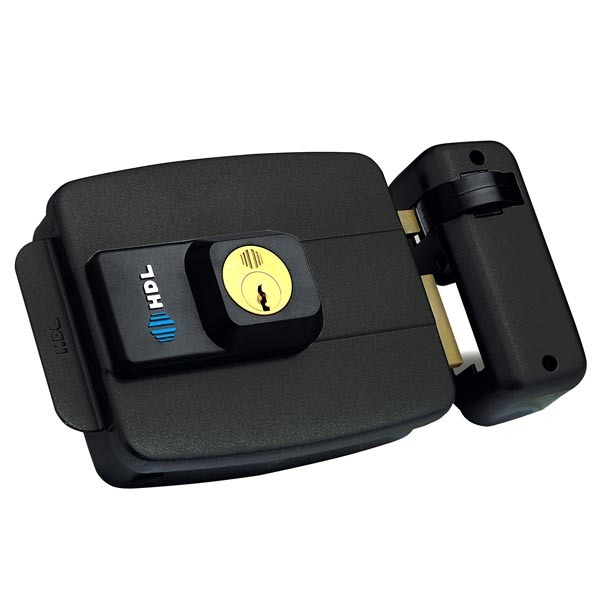
\includegraphics[scale=.25]{imagens/eletrica}
	\\\textbf{Fonte:} \href{https://www.leroymerlin.com.br/fechadura-eletrica-c-90-ajustavel-12v-preto-hdl_86491860}{Leroy Merlin}
	\label{fig:eletrica}
\end{figure}
\FloatBarrier

\FloatBarrier
\begin{figure}[!htbp]
	\centering
	\caption{Fechadura Biométrica}
	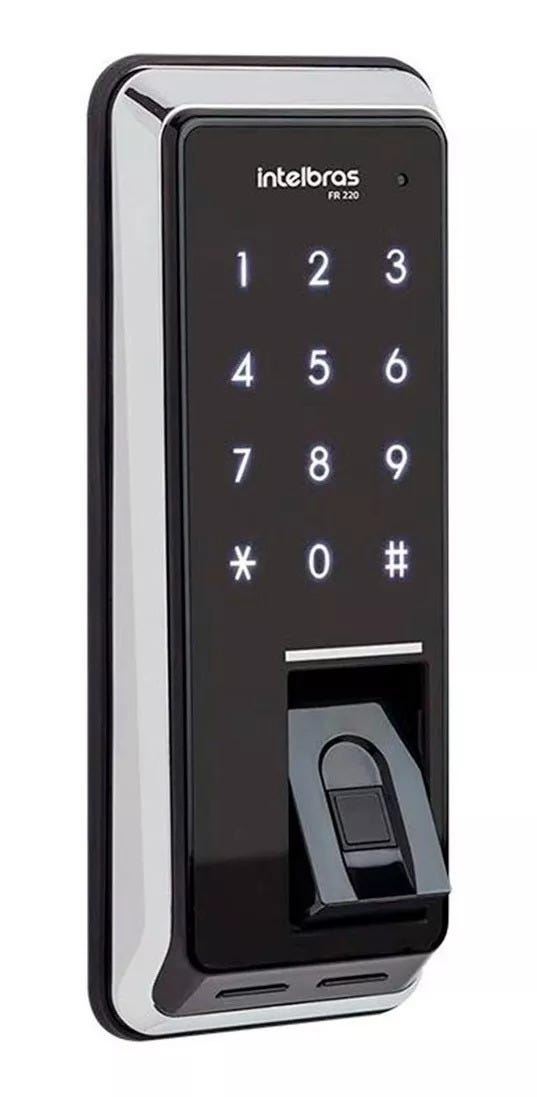
\includegraphics[scale=.15]{imagens/biometrica}
	\\\textbf{Fonte:} \href{https://www.madeiramadeira.com.br/fechadura-digital-fr220-acesso-por-biometrica-prox-senha-1560519.html}{Madeira Madeira}
	\label{fig:biometrica}
\end{figure}
\FloatBarrier

\section{Objetivos}
O objetivo deste projeto é desenvolver uma fechadura
eletrônica utilizando sensor de RFID visando menor
custo de produção e maior aproveitamento dos componentes
utilizados. A fechadura deverá manter salvo os usuários e
possuir um usuário administrador que pode cadastrar ou remover usuários.

Além disso, o projeto busca incentivar nos participantes a busca por
conhecimentos necessários de forma autônoma, sem que essa informação seja passada a
eles de forma passiva. 

\section{Justificativa}
Essa montagem foi escolhida pelo grupo devido à falta de segurança das
fechaduras comuns e alto preço de fechaduras eletrônicas no mercado. Então a busca por
materiais de baixo custo para tornar o produto mais acessível para o consumidor final é
parte determinante para o sucesso do projeto

\section{Metodologia}
O projeto ocorrerá principalmente em duas etapas: pesquisa e montagem.

Na parte de pesquisa os conhecimentos necessários para a criação da fechadura
serão buscados pelos alunos sendo utilizada a ajuda de livros, internet e dos
professores. Além disso, será necessário buscar pelos melhores componentes para
serem utilizados, para garantir assim o melhor custo-benefício.

Na etapa de montagem serão feitos dois protótipos e uma montagem final. Os
protótipos serão feitos para o teste e melhor conhecimento do sensor e do 
atuador e serão remontados até que funcionem perfeitamente.

\begin{itemize}
\item Protótipo 1: Tem como objetivo a verificação do funcionamento do
microcontrolador (ATMEGA 328p) aliado a forma de abertura da
fechadura (RFID)

\item Protótipo 2: O atuador (eletroímã) será adicionado ao protótipo e a
fechadura será apresentada.

\item Projeto final: A fechadura pronta será apresentada com todas as suas
funcionalidades e interfaces.
\end{itemize}